\section{Companion relations}\label{sec:comp-rel}

In $\CMSO$, it is not possible to guess relations on the vertices of graphs in general. In this section, we present a very particular case of relations which can be guessed in $\CMSO$,  called \emph{companion relations}.

    \begin{definition}[Paths]
   A \emph{path} $p$ of $G$ is a non-repeating list $(v_0,e_1,v_1,\dots,e_n,v_n)$ where $v_i$ is a vertex of $G$ and $e_i$ is an edge of $G$, such that the interface of $e_i$ is either $(v_{i-1}, v_{i})$ or $(v_{i},v_{i-1})$, for every $i\in[1,n]$. The path $p$ is \emph{directed} if the interface of $e_i$ is  $(v_{i-1}, v_{i})$ for every $i\in[1,n]$. The vertex $v_0$ is the \emph{input} of $p$, $v_n$  is its \emph{output} and $(v_0,v_n)$ its \emph{interface}. 
   \end{definition} 


\begin{definition}[Companion relation] Let $G$ be a graph. 
Two paths  of $G$ are \emph{orthogonal} if they do not share any edge, and whenever they share a vertex, it is necessarily an interface vertex of one of them. %A set of paths is a \emph{set of orthogonal paths} if its paths are pairwise orthogonal.

A relation $R$ on the vertices of $G$ is a \emph{companion relation} if there is a set of (pairwise) orthogonal paths $P$ such that $(v,w)\in R$ iff $(v,w)$ is the interface of a path $p\in P$. We say that $p$ is a \emph{witness} for $(v,w)$, and that $P$ is a \emph{witness} for the relation $R$.
\end{definition}

\begin{example} \label{ex:guared-set-of-paths}
The relation indicated by the green dotted arrows below is a companion relation. This is not the case for the one indicated by the red dotted arrows.
\begin{center}
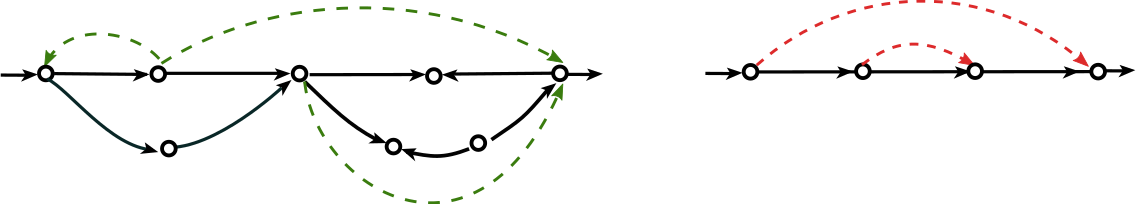
\includegraphics[scale=.4]{Pictures/guarded-set-of-paths}
\end{center}
 \end{example}

We introduce $\CMSO^r$, an extension of $\CMSO$ where quantification over companion relations is possible.

\begin{definition}[The logic $\CMSO^r$] 
  Let $\mathbb{X}_r$ be a set of \emph{relation variables}, whose elements are denoted $R, S, \dots$. The formulas of $\CMSO^r$ are of the following form:
\begin{align*}
 \phi :=&\ \CMSO\ |\ \exists R.\ \phi\ |\ (x,y)\in R & \qquad (R\in \mathbb{X}_r,\ x,y\in\mathbb{X}_1).
\end{align*}
\end{definition}
 
 As for $\CMSO$, we need to define the semantics of a formula over pointed graphs to handle free variables.
 
\begin{definition}[Semantics of $\CMSO^r$]
Let $G$ be a graph and $\Gamma$ be a set of variables.  An interpretation of $\Gamma$ is as usual, but here every relation variable is mapped to a binary relation on the vertices of $G$.  We define the \emph{satisfiability relation} $\langle G, I\rangle\models \phi$ as usual, by induction on the formula $\phi$. The only new cases are the quantification  $\exists R$ which is interpreted as ``there exists a companion relation $R$ on the vertices of the graph'', and the formulas $(x,y)\in R$ which are interpreted as ``there is a pair of vertices $(x,y)$ in $R$''. 
\end{definition}


\subsection{The logic $\CMSO^r$ have the same expressive power as $\CMSO$}
%A \emph{path} in a graph is a non-empty connected module, which becomes disconnected when we remove one of its edges. A \emph{directed path}, is path whose  vertices can be totally ordered (the input being the least element and the output the greatest element), such that each consecutive vertices are connected by an edge from the smallest to the biggest.



To guess a companion relation in $\CMSO$, we show how to encode a set of guarded paths by a collection of sets called a \emph{footprint}.


\begin{definition}[Frontier edges of a path] Let $p=(v_0,e_1,v_1,\dots,e_n,v_n)$ be a path. If $n>1$, we call $e_1$ the \emph{opening edge} of $p$ and $e_n$ its \emph{closing edge}. If $n=0$, we call $e_0$ its \emph{single edge}.  Opening, closing and single edges are called the \emph{frontier edges} of $p$, the other edges are called its \emph{inner edges}.  
 \end{definition}


 
 \begin{definition}[Footprint] A \emph{footprint} in a graph $G$  is the following collection of data: a partition of the vertices of $G$ into \emph{non-path} and \emph{path} vertices, a partition of edges into \emph{non-path} and \emph{path} edges, a partition of path edges into \emph{frontier} and \emph{inner} edges, a partition of frontier edges into \emph{opening, closing and single} edges and a partition of path edges into \emph{direct} and \emph{inverse} edges.
 
 The partition of path edges into direct and inverse ones provides them with a new orientation:  they conserve their original  orientation if they are direct, or get reversed (we swap the source and target) if they are inverse edges.  
 
 Let $\mathbb{F}$ be a footprint. A path $p$ is encoded by $\mathbb{F}$  if its edges and vertices are path edges and path vertices of $\mathbb{F}$,  if its inner, frontier, opening, closing and single edges are edges of the corresponding sets in $\mathbb{F}$.  Moreover, $p$ must form a directed path with the new orientation dictated by $\mathbb{F}$. 
 \end{definition}
 
%\begin{remark}\label{rmk:Encoding-CMSO}
%The main interest of paths encoding is that they are a collection of sets of edges and vertices, hence they can be guessed in $\CMSO$. Once we guess a paths encoding $\mathbb{F}$, we can express in $\CMSO$ that a module $(s,Z,t)$ is a path encoded by $\mathbb{F}$, and that the set of paths encoded by $\mathbb{F}$ is guarded. 
% \end{remark}


\begin{example} We represent below a footprint in the left graph of Ex.~\ref{ex:guared-set-of-paths}. Non-path edges and vertices are  grey, path vertices are  black, opening edges are green, closing edges are yellow, single edges are pink and all the other inner edges are black. For path edges, we display the new orientation induced by the footprint instead of the original one. The set of paths encoded by this footprint are a witness that the green relation of Ex.~\ref{ex:guared-set-of-paths} is a companion relation. 
   \begin{center} 
 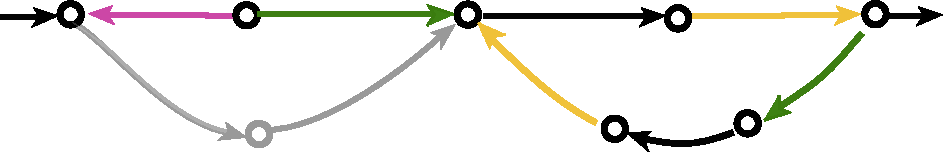
\includegraphics[scale=.45]{Pictures/encoding-set-of-paths.pdf}
 \end{center}
 \end{example}
  
 \begin{proposition}\label{prop:encoding-guarded-sets-of-paths}
 Let $G$ be a graph and $P$ a set of orthogonal paths of $G$. There is a footprint $\mathbb{F}$ such that $P$ is the set of paths encoded by $\mathbb{F}$.
\end{proposition} 
\begin{proof}
 We define $\mathbb{F}$ as the natural paths encoding associated to $P$: its path edges and path vertices are respectively the set of edges and vertices that appear in the paths of $P$, its frontier, inner, opening, closing and simple edges are the corresponding edges in the paths of $P$. Notice that it is possible reorient the edges of every path so that it becomes directed. Since the paths of $P$ do not share any edge, we can reorient their edges consistently in order to make them directed. We define direct edges as the path edges whose orientation did not change after this operation,  and inverse edges the remaining path edges.
\smallskip

It is clear that the paths of $P$ are encoded by $\mathbb{F}$, let us show that they are the only ones. We start by stating the following claim which follows from the definitions.
\begin{claim}\label{claim}
Let $p$ be a path in $P$ and $v$ a vertex of $p$. If $v$ is the source (w.r.t. the new orientation induced by $\mathbb{F}$) of an inner edge or the closing edge of $p$, then, by construction, $v$ cannot be an interface vertex of $p$. If $v$ is the target (w.r.t. the new orientation induced by $\mathbb{F}$) of an inner edge or the opening edge of $p$, then by construction, $v$ cannot be an interface vertex of $p$.
\end{claim}
Let $p$ be a path encoded by $\mathbb{F}$. If $p$ has a unique edge, then it is a single edge, and by construction single edges come exclusively from paths of $P$ with a unique edge. In this case, $p$ is clearly a path in $P$. 

Suppose now that $p$ has at least two edges. The opening edge of $p$ is, by construction, the opening edge of some path $q$ of $P$. Let $v$ be the vertex of $p$ such that all the vertices between the input of $p$ and $v$ are also vertices of $q$ and the successor of $v$ in $p$, call it $w$, is not a vertex of $q$. 

By Claim~\ref{claim}, and since $v$ is the target of the opening edge or an inner edge of the path $q$, it is not an interface vertex of $q$.

Let $e$ be the edge  from $v$ to $w$ in the path $p$. The edge $e$ is either an inner edge or a closing edge, and by construction, there is a path $r$ of $P$ containing this edge. By Claim~\ref{claim}, and since $v$ is the source of an inner edge or the closing edge of $r$, we have that $v$ is not an interface vertex of $r$. 

Here is a picture illustrating this construction, where the path between $\iota$ and $o$ is $p$.
\begin{center}
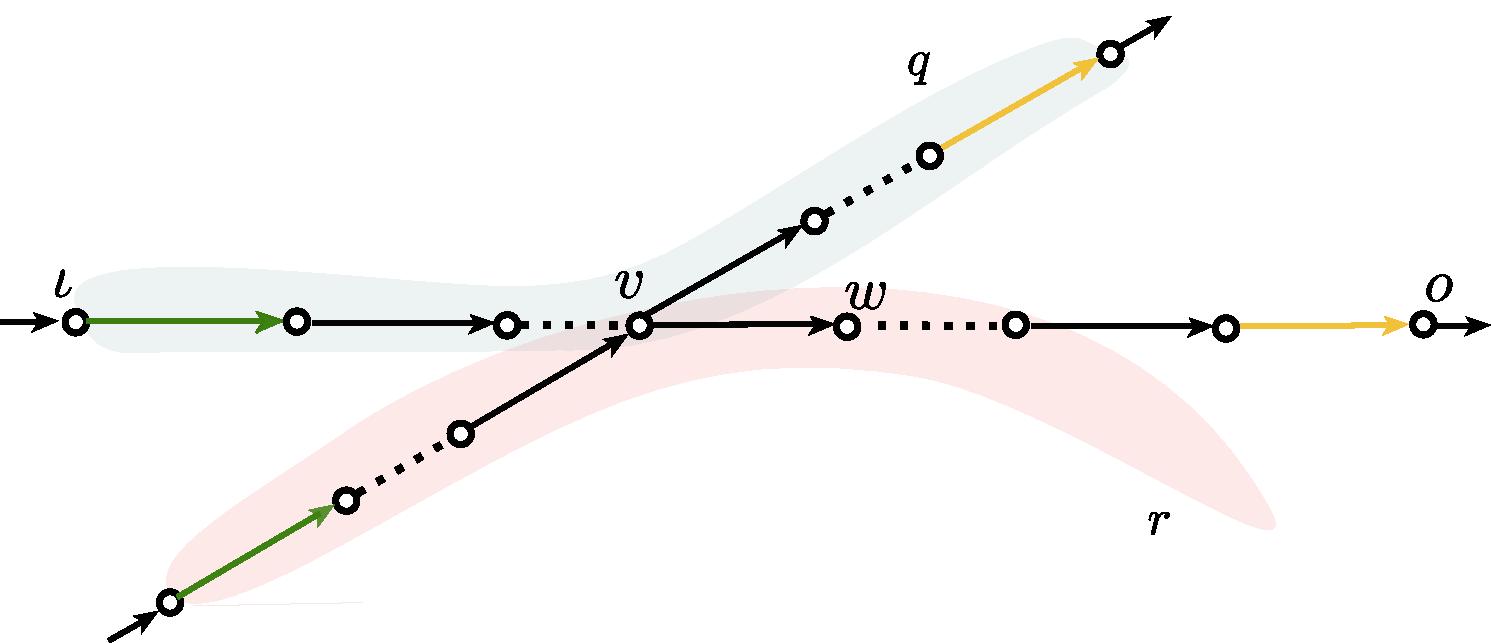
\includegraphics[scale=.3]{Pictures/proof-encoding-paths}
\end{center}
We have found two paths of $P$, $q$ and $r$, sharing a vertex $v$ which is an interface vertex of none of them. This yields a contradiction. 
\end{proof}

\begin{theorem}
If a language is $\CMSO^r$ definable then it is $\CMSO$ definable.
\end{theorem}

\begin{proof}
Let $\phi$ be a $\CMSO^r$ formula. We transfor $\phi$ into a $\CMSO$ formula $\psi$ as follows. We replace every quantification $\exists R.$ by a sequence of existential sets quantifications representing  a footprint $\mathbb{F}$. 

Saying that a subgraph $(s,Z,t)$ is a directed path is expressible in $\CMSO$, and checking that its different components (frontier vertices, opening and closing edges, etc) match the footprint is also easily expressible in $\CMSO$. Hence we can define a  $\CMSO$ formula $\mathsf{encoded\text{-}path}_\mathbb{F}(s,Z,t)$ which says that $(s,Z,t)$ is a path encoded by $\mathbb{F}$. 

We replace every  subformula of $\phi$ of the form ``$(s,t)\in R$'' by the following formula: $$\exists Z.\ \mathsf{encoded\text{-}path}_\mathbb{F}(s,Z,t)$$
\end{proof}
